
% \documentclass[final,5p,times]{elsarticle}
\documentclass[final,5p,times,twocolumn]{elsarticle}


\usepackage{graphicx}%
\usepackage{multirow}%
\usepackage{amsmath,amssymb,amsfonts}%
\usepackage{amsthm}%
\usepackage{mathrsfs}%
\usepackage[title]{appendix}%
\usepackage{xcolor}%
\usepackage{textcomp}%
\usepackage{manyfoot}%
\usepackage{booktabs}%
\usepackage{algorithm}%
\usepackage{algorithmicx}%
\usepackage{algpseudocode}%
\usepackage{listings}%
\usepackage{threeparttable}%

%% The amsthm package provides extended theorem environments
% \usepackage{amsthm}

%% The lineno packages adds line numbers. Start line numbering with
%% \begin{linenumbers}, end it with \end{linenumbers}. Or switch it on
%% for the whole article with \linenumbers.
%% \usepackage{lineno}

\journal{Journal of \LaTeX\ Templates}

\begin{document}

\begin{frontmatter}

    \title{Area-Throughput Efficient Implementations of CRAFT Cipher For Internet of Things }

    \author[a,b]{Jiahao Xiang}
    \author[a,b]{Lang Li\corref{cor1}}

    \ead{lilang911@126.com}

    \cortext[cor1]{Corresponding author}

    \affiliation[a]{organization={College of Computer Science and Technology},%Department and Organization
        addressline={Hengyang Normal University},
        city={Hengyang},
        postcode={421002},
        state={},
        country={China}}

    \affiliation[b]{organization={Hunan Provincial Key Laboratory of Intelligent Information Processing and Application},%Department and Organization
        addressline={Hengyang Normal University},
        city={Hengyang},
        postcode={421002},
        state={},
        country={China}}



    \begin{abstract}
        The Internet of Things (IoT) has revolutionized device and data interactions, enabling unparalleled connectivity and automation. However, the resource limitations of many IoT devices create challenges for implementing robust security measures. Lightweight cryptography, a cryptography subset, offers solutions tailored for these resource-constrained devices.
        This paper presents two optimized designs for the CRAFT lightweight block cipher: Serial and Unrolled. The Serial design reduces the data width and the number of components, thereby enhancing efficiency. In contrast, the Unrolled design aims to decrease latency, ensuring quicker processing. Boolean satisfiability (SAT) solvers are used to determine the optimal implementation of the Sub-Box.
        The proposed designs were evaluated on three different FPGA platforms: Artix-7, Kintex-7, and Spartan-7. The results show that the Serial design significantly reduces area usage compared to the PRESENT cipher. On the other hand, the Unrolled design substantially improves the throughput rate. Additionally, the Unrolled design markedly reduces energy consumption per bit compared to the PRESENT cipher.
        These results suggest that the proposed designs could potentially improve the security and efficiency of IoT devices.
    \end{abstract}


    \begin{keyword}
        %% keywords here, in the form: keyword \sep keyword
        Lightweight block cipher \sep Internet of Things  \sep Field-programmable gate array(FPGA)\sep  Low-area, High-throughput
        %% PACS codes here, in the form: \PACS code \sep code

        %% MSC codes here, in the form: \MSC code \sep code
        %% or \MSC[2008] code \sep code (2000 is the default)
    \end{keyword}

\end{frontmatter}

%% \linenumbers

%% main text


\section{Introduction}\label{sec1}

The Internet of Things (IoT) is making rapid strides into various sectors such as personal health care, environmental monitoring, home automation, smart mobility, and Industry 4.0. As security concerns continue to surface, they are thoroughly discussed in \cite{Meneghello2019a}. The most effective way to ensure data protection is by employing the cryptography techniques outlined in \cite{Swessi2022}.

However, the resource constraints of many IoT devices pose challenges for the implementation of robust security measures. These devices often have limited memory, processing power, and energy. Therefore, the security measures need to be lightweight to ensure they do not overburden the resources. Lightweight cryptography, a subset of cryptography, provides solutions specifically designed for these resource-limited devices, as discussed in \cite{Mohajerani2020}.

The lightweight cryptography have been widely studied in recent years, such as PRESENT \cite{Bogdanov2007}, LED \cite{Guo2011}, Midori \cite{Banik2015a}, QTL \cite{Li2016}, GIFT \cite{Banik2017}, CRAFT \cite{Beierle2019}, Shadow \cite{Guo2021}, DULBC \cite{Yang2022},IVLBC \cite{Huang2023}, BipBip \cite{Belkheyar2023} and LELBC \cite{Song2024}. more cipher can be found in \cite{Zakaria2023}.

ISO/IEC 29192-2, a standard for lightweight cryptography, offers a set of algorithms that are suitable for these resource-constrained environments. Yet, the PRESENT algorithm, included in this standard, was break by differential fault analysis (DFA). This has led to a demand for a new lightweight block cipher to replace PRESENT. The CRAFT cipher was designed to resist DFA and was published in Fast Software Encryption (FSE).

In this work, we propose the three architectures of FPGA implementations for the CRAFT \cite{Beierle2019}, respectively Round based, Serial, and Loop unrolled.
This allows IoV practitioners to select the architectures that best suit their needs.
The contributions of this article can be summarized as follows.

The rest of this article is organized as follows.
Section~\ref{sec2} presents specification of CRAFT; the proposed the three architectures of FPGA implementations for the CRAFT are present in Section 3; Section 4 presents the implementation results, analysis, and comparison with other similar works; finally, the work is concluded in Section 5.

\section{Specification of CRAFT}\label{sec2}

All notations used in this paper are shown in Table~\ref{tab1}.
CRAFT is a lightweight tweakable block cipher made out of involutory building blocks.
It consists of a 64-bit block, a 128-bit key, and a 64-bit tweak. In this cipher, a 64-bit input plaintext $P$ is transformed into a 64-bit output ciphertext $C$ using a 128-bit key $K$ and a 64-bit tweak $T$. Figure~\ref{fig1} shows the structure of CRAFT.


\begin{table}[h]
    \centering
    \caption{Notations used in this paper}\label{tab1}%
    \begin{tabular}{|c|c|}
        \hline
        Notation & Description                                 \\
        \hline
        $TK$     & 64-bit tweakeys                             \\
        $RC_i$   & 64-bit round constant in the $i^{th}$ round \\
        \hline
    \end{tabular}
\end{table}

\begin{figure}[h]%
    \centering
    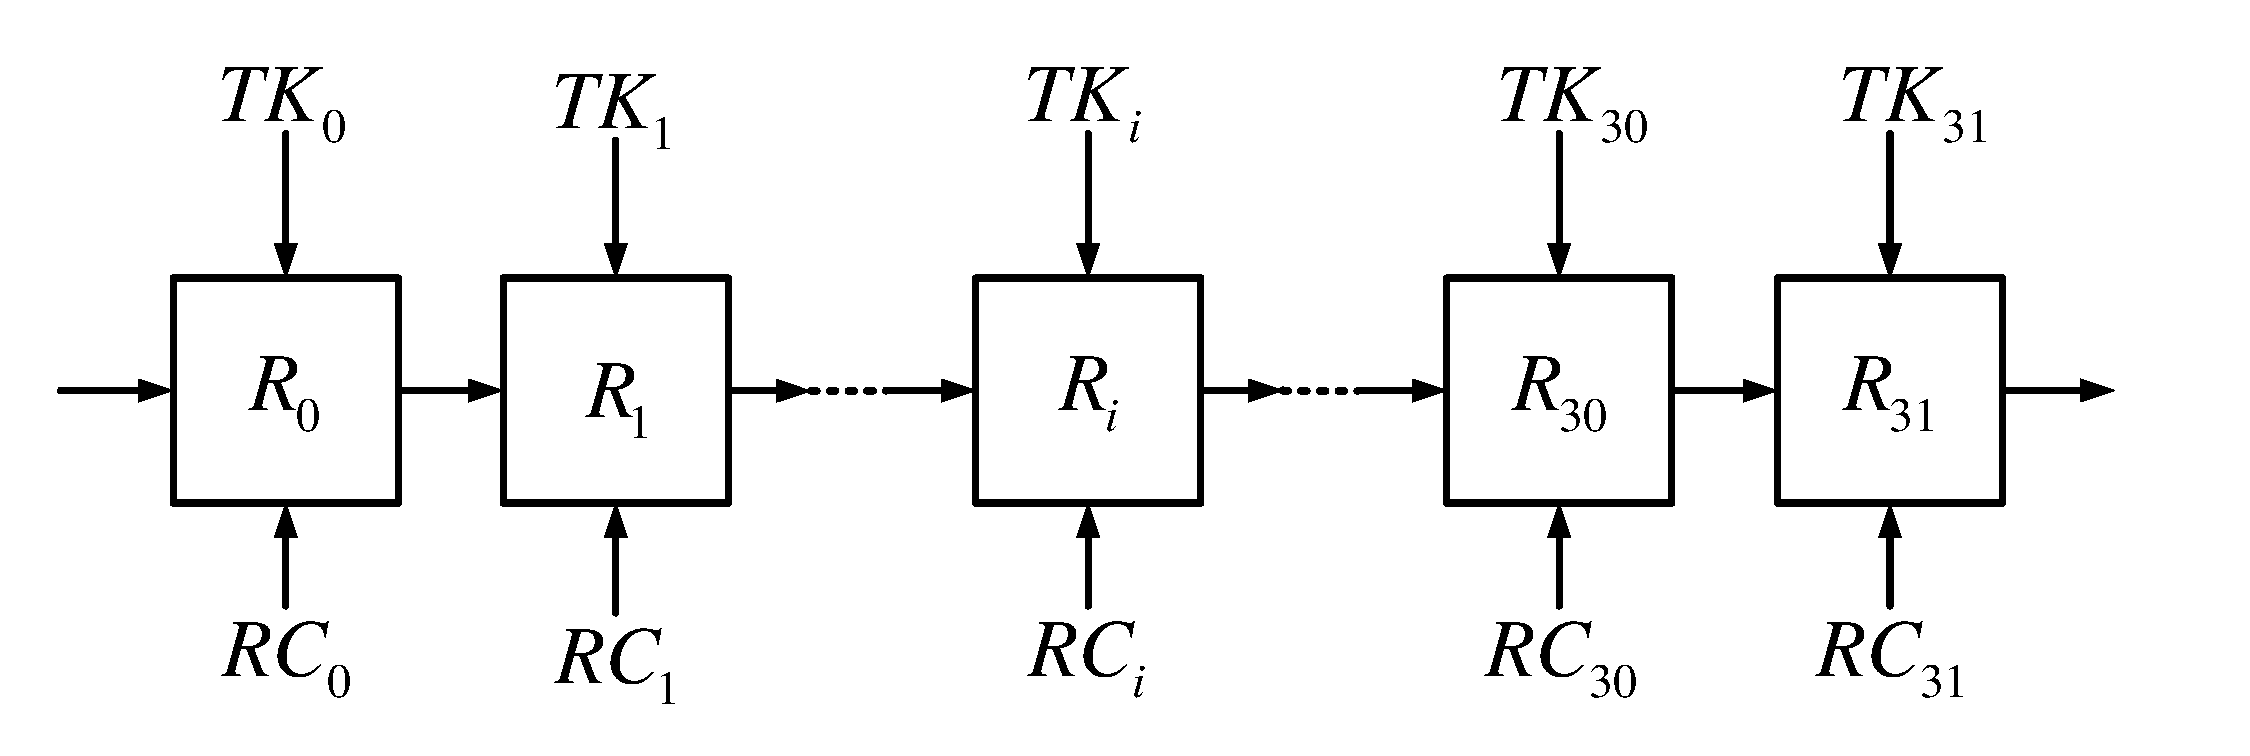
\includegraphics[width=0.45\textwidth]{./fig/struct-craft.pdf}
    \caption{Structure of CRAFT}\label{fig1}
\end{figure}

\section{Implementations}\label{sec3}

For the first time, the components of CRAFT have been optimized to achieve efficient area and throughput, resulting in two proposed implementation architectures: Serial and Unrolled.


\subsection{Serial Architecture (A1)}\label{subsec2}
Compared to round-based architectures, serial architectures can significantly reduce area usage by reusing components. For instance, the number of Sub-Boxes is reduced from 16 to 1. The clock gating technique is also employed to enable each component and minimize the energy consumption of encryption. The proposed architecture is presented in Figure~\ref{fig3}.

The design includes one Sub-Box, one 4-bit Mix-columns, and two register banks for storing keys (referred to as Key-Register) and plaintext (referred to as State-Register). These also act as temporary registers for storing intermediate results. To store intermediate results into the State-Register bank, the design includes one feedback path. The PermuteNibbles is incorporated into the State-Register bank.

It's worth noting that the execution of permute requires 64-bit. To reuse the State-Register block, the order of execution of Sub-Box and Permute is altered. Additionally, the first round of the encryption process avoids the Permute operation through the control signal, ensuring the correctness of the encryption algorithm.

\begin{figure*}[h]%   
    \centering
    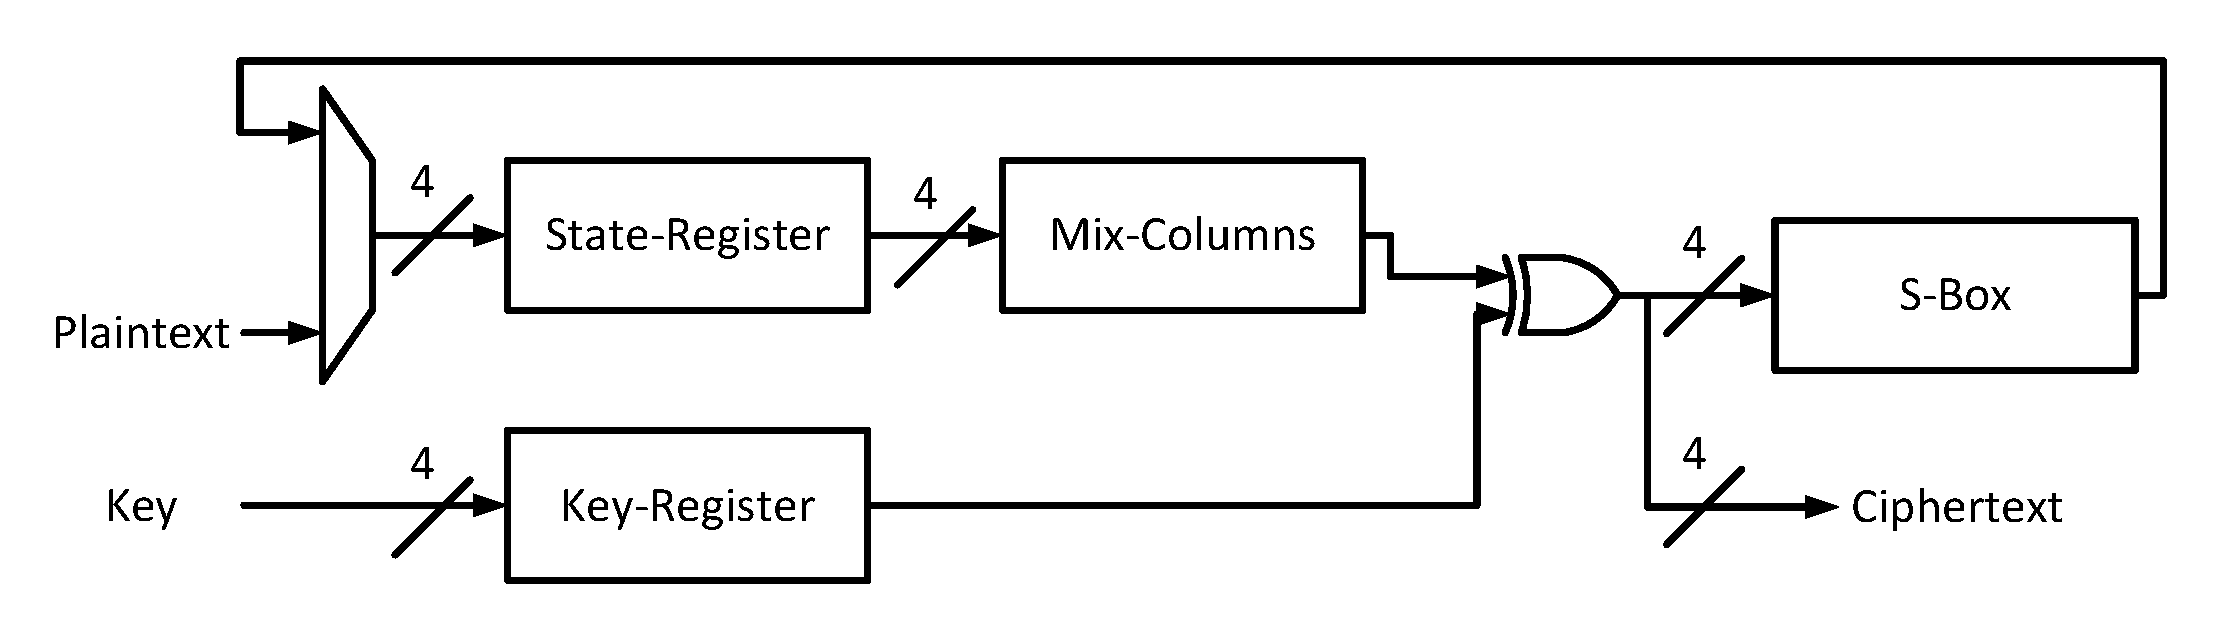
\includegraphics[width=0.7\textwidth]{./fig/serial-archticture.pdf}
    \caption{Serial architecture of CRAFT}\label{fig3}
\end{figure*}


\subsubsection{Sub-Box Optimization }\label{subsubsec1}


Sub-Box provides a confusing characteristic for the entire encryption algorithm, however it requires a large amount of area.
There are different methods of implementation of Sub-Box.
The most popular implementation is using a lookup table (LUT), such as \cite{DBLP:journals/tcas/Lara-NinoDM17}.
However it uses a lot of flip-flop, which will bring a lot of area consumption.
Using Sub-Box's equivalent logical expression for this will reduce area consumption, such as \cite{bao2019peigen}, \cite{bib16}.

Boolean satisfiability (SAT) solvers can be used to find Sub-Box that satisfy certain implement, such as being resistant to software or hardware implement.
In more detail, the Sub-Box implement can be encoded as Boolean constraints by representing the Sub-Box as a truth table and then using Boolean variables to represent the input and output bits of the Sub-Box.
The constraints can then be formulated based on the desired implement of the Sub-Box.
Once the Sub-Box implement are encoded as Boolean constraints, a SAT solver can be used to find a satisfying assignment to these constraints, which corresponds to an Sub-Box that satisfies the desired implement.

The gate equivalent complexity(GEC) of a SAT instance is the number of logical gates required to implement the Boolean formula that represents the instance.
GEC can be calculated by converting the Boolean formula into a circuit of logical gates, such as AND, OR, and NOT gates.
The number of gates in the circuit corresponds to the GEC of the instance.

In our design, we optimize and use GEC encoding scheme of \cite{bib16} to implement the Sub-Box.
Our encoding scheme as follows in Equations~\ref{eq1}:



% \begin{align*}
% \begin{split}

\begin{flalign}
    \forall i \in & \{0,1,\ldots ,K-1\}: \nonumber                                                                        \\
    T_i =         & F_{if} (BB_i[0], \thicksim (Q_{4i} \cdot Q_{4i+1}) \cdot \thicksim Q_{4i+2} \cdot Q_{4i+3}) \nonumber \\
                  & + F_{if} (BB_i[1], Q_{4i+2} \cdot (Q_{4i} + Q_{4i+1})) \nonumber                                      \\
                  & + F_{if} (BB_i[2], Q_{4i} \cdot Q_{4i+1} \cdot Q_{4i+2})  \label{eq1}                                 \\
                  & + F_{if} (BB_i[3], Q_{4i+2}) + F_{if} (BB_i[4], Q_{4i}) \nonumber                                     \\
                  & + F_{if} (BB_i[5], Q_{4i} \cdot Q_{4i+1}) \nonumber                                                   \\
                  & + F_{if} (BB_i[6], Q_{4i} + Q_{4i+1}) + F_{if} (BB_i[7], max) \nonumber
\end{flalign}



where $K$ is numbers of the logical gates, $Q_{4i}-Q_{4i+3}$ is the input of the $i^{th}$ logical gate, $T_i$ is the output of the $i^{th}$ logical gate, and $F_{if}$ is a function that returns the value of the second argument if the first argument is true and returns the value of zero otherwise.
The value of $max$ is all one's in the binary expression, which is represented logically as an inverse.
$BB_i$ represents the type of the $i^{th}$ logical gate, which is a 8-bit binary number. The different types of logical gate used in this encoding scheme are listed in Table~\ref{tab3}.


The optimized scheme of Sub-Box is shown in Equations~\ref{eq2}, where $X_0-X_3$ is the input of the Sub-Box and $Y_0-Y_3$ is the output of the Sub-Box.
The proposed scheme of Sub-Box is implemented by four MOAI1 gates, three MAOI1 gates, and one AND3 gate.
This module of the proposed Sub-Box reduced the area by 28.9\% with \cite{bao2019peigen} (based on gate equivalent estimation on UMC 180nm library).

\begin{align}
    T_0 & = \text{MAOI1}(X_0, X_1, X_0, X_1) \nonumber          \\
    T_1 & = \text{AND3}(X_3, X_2, X_3) \nonumber                \\
    T_2 & = \text{MAOI1}(X_1, X_2, X_0, X_3) \nonumber          \\
    T_3 & = \text{MOAI1}(X_1, X_0, X_2, X_2) \nonumber          \\
    T_4 & = \text{MOAI1}(X_3, T_0, T_3, T_3) \label{eq2}        \\
    T_5 & = \text{MOAI1}(T_3, T_0, X_0, T_1) \nonumber          \\
    T_6 & = \text{MAOI1}(X_0, T_0, X_3, T_0) \nonumber          \\
    T_7 & = \text{MOAI1}(X_0, T_1, T_2, T_2) \nonumber          \\
    Y_0 & = T_5 \quad Y_1 = T_7 \quad Y_2 = T_6 \quad Y_3 = T_4
    \nonumber
\end{align}


\begin{table}[h]
    \caption{Encoding of different types of logical gate}\label{tab3}%
    \begin{tabular}{|c|c|c|}
        \hline
        logical expression                                   & $BB_i$[0:7]     & gate type \\
        \hline
        $Q_0 \oplus Q_1$                                     & 0 0 0 0 0 0 1 0 & XOR       \\
        $\sim (Q_0 \oplus Q_1)$                              & 0 0 0 0 0 0 1 1 & XNOR      \\
        $Q_0 \land Q_1$                                      & 0 0 0 0 0 1 0 0 & AND       \\
        $\sim (Q_0 \land Q_1)$                               & 0 0 0 0 0 1 0 1 & NAND      \\
        $Q_0 \lor Q_1$                                       & 0 0 0 0 0 1 1 0 & OR        \\
        $\sim (Q_0 \lor Q_1)$                                & 0 0 0 0 0 1 1 1 & NOR       \\
        $\sim Q_0$                                           & 0 0 0 0 1 0 0 1 & NOT       \\
        $\sim Q_1$                                           & 0 0 0 0 1 0 1 1 & NOT       \\
        $\sim Q_2$                                           & 0 0 0 1 0 0 0 1 & NOT       \\
        $Q_0 \oplus Q_1 \oplus Q_2$                          & 0 0 0 1 0 0 1 0 & XOR3      \\
        $\sim (Q_0 \oplus Q_1 \oplus Q_2)$                   & 0 0 0 1 0 0 1 1 & XNOR3     \\
        $Q_0 \land Q_1 \land Q_2$                            & 0 0 1 0 0 0 0 0 & AND3      \\
        $\sim (Q_0 \land Q_1 \land Q_2)$                     & 0 0 1 0 0 0 0 1 & NAND3     \\
        $Q_0 \lor Q_1 \lor Q_2$                              & 0 1 1 1 0 1 1 0 & OR3       \\
        $\sim (Q_0 \lor Q_1 \lor Q_2)$                       & 0 1 1 1 0 1 1 1 & NOR3      \\
        $\sim ((Q_0 \land Q_1) \lor (\sim (Q_2 \lor Q_3)))$  & 1 0 1 1 0 0 0 0 & MAOI1     \\
        $\sim (\sim (Q_0 \land Q_1) \land ((Q_2 \lor Q_3)))$ & 1 0 1 1 0 0 0 1 & MOAI1     \\
        \hline
    \end{tabular}
\end{table}

\subsubsection{Mix-Columns Optimization}\label{subsubsec2}

The Mix-Columns component is a linear transformation of the input column.
The input column is multiplied by a constant matrix $M$ to produce the output column.
$M$ is a involutory matrix, which means $M^2 = E$, where $E$ is the identity matrix.
It is easy to decrypt the ciphertext by multiplying the ciphertext with $M$ again.
The Mix-columns component is shown in Equation~\ref{eq3}.
where $I_{0,j}$, $I_{1,j}$, $I_{2,j}$, and $I_{3,j}$ are the input column, $I'_{0,j}$, $I'_{1,j}$, $I'_{2,j}$, and $I'_{3,j}$ are the output column, and $j$ is the column index, $j \in \{0,\dots,3\}$.

\begin{equation}
    \begin{bmatrix}
        I'_{0,j} \\
        I'_{1,j} \\
        I'_{2,j} \\
        I'_{3,j}
    \end{bmatrix}
    =
    \begin{bmatrix}
        1 & 0 & 1 & 1 \\
        0 & 1 & 0 & 1 \\
        0 & 0 & 1 & 0 \\
        0 & 0 & 0 & 1
    \end{bmatrix}
    \begin{bmatrix}
        I_{0,j} \\
        I_{1,j} \\
        I_{2,j} \\
        I_{3,j}
    \end{bmatrix}
    \label{eq3}
\end{equation}


In order to reduce the area of this component, the serial architecture of Mix-Columns is utilized, as shown in Figure~\ref{serial_mix_columns_fig}.
The serial architecture of Mix-Columns requires four 4-bit registers, two multiplexers, and three XOR gates.
The operation of Mix-Columns involves three distinct stages: freeze, shift, and add.
During the freeze stage, the register values are kept unchanged by setting both $CM_0$ and $CM_1$ to 0.
In the shift stage, a shift in the register values from $RM_0$ to $RM_4$ is induced by setting both $CM_0$ and $CM_1$ to 1.
Finally, in the add stage, an addition operation on the column values is executed according to Equation~\ref{eq3}. This is achieved by setting $CM_0$ and $CM_1$ to 0 and 1, respectively.

The timing diagram for the serial architecture of Mix-Columns is depicted in Figure~\ref{serial_time_diagrm_mix_colunms}.
It requires five clock cycles to compute the next columns from the previous ones, and an additional four clock cycles to transfer data from the internal register of Mix-Columns to the State-Register.
Therefore, a complete state round requires a total of 36 clock cycles.


\begin{figure}[h]%   
    \centering
    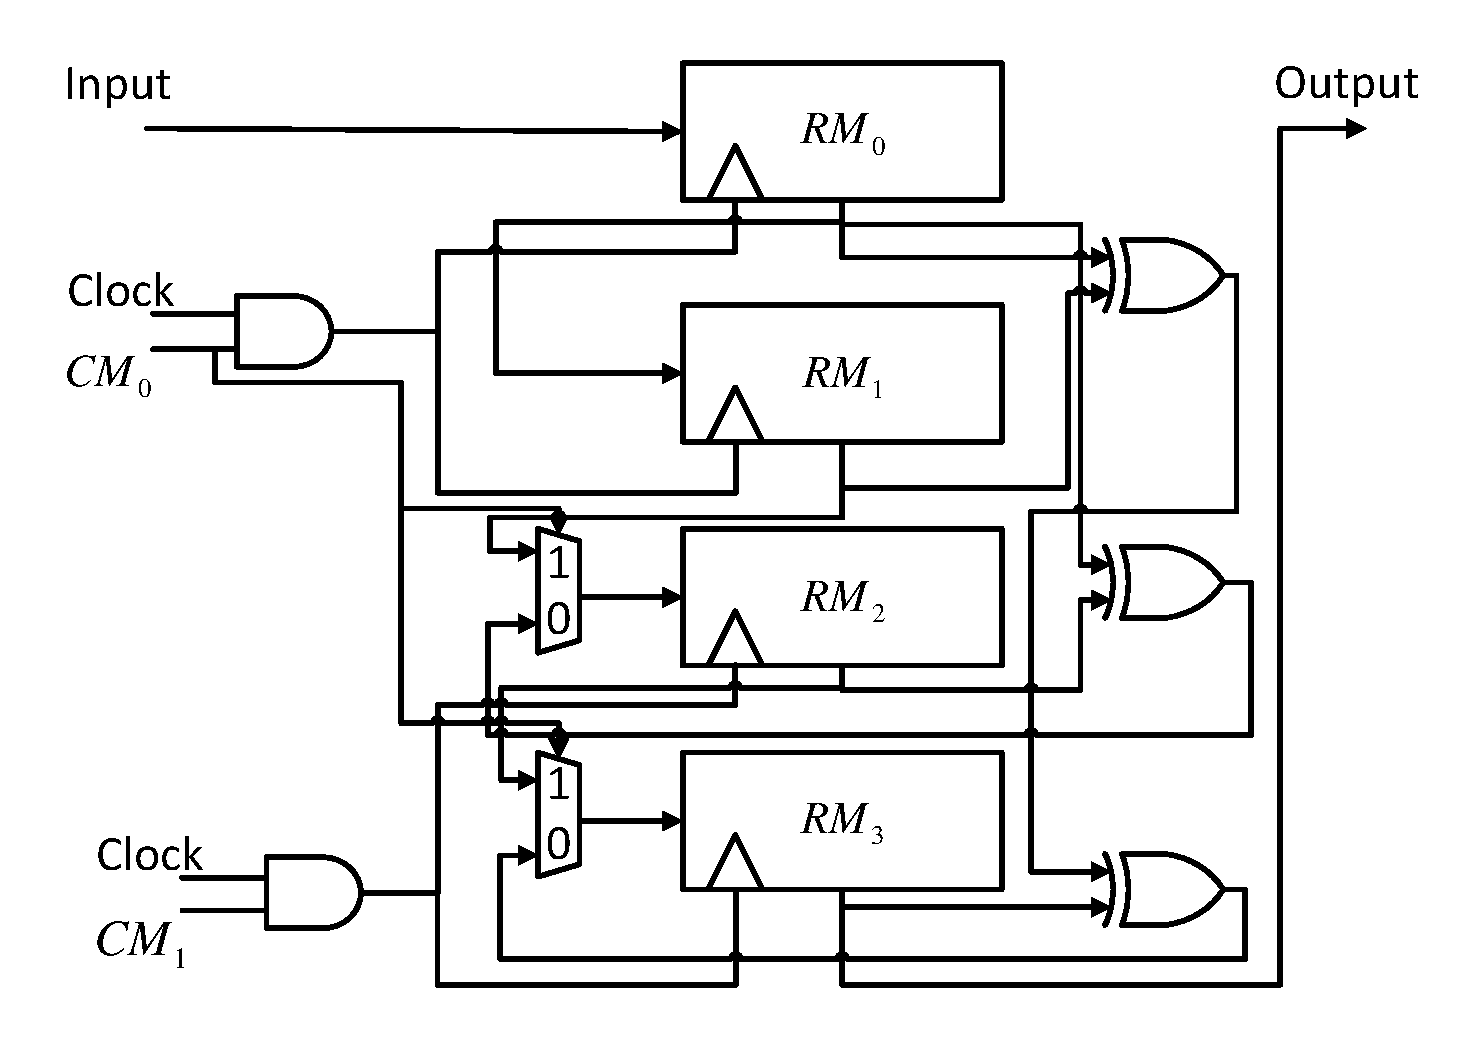
\includegraphics[width=0.5\textwidth]{./fig/Mix-Columns.pdf}
    \caption{Serial Architecture of Mix-Columns with clock gating}\label{serial_mix_columns_fig}
\end{figure}

\begin{figure}[h]%   
    \centering
    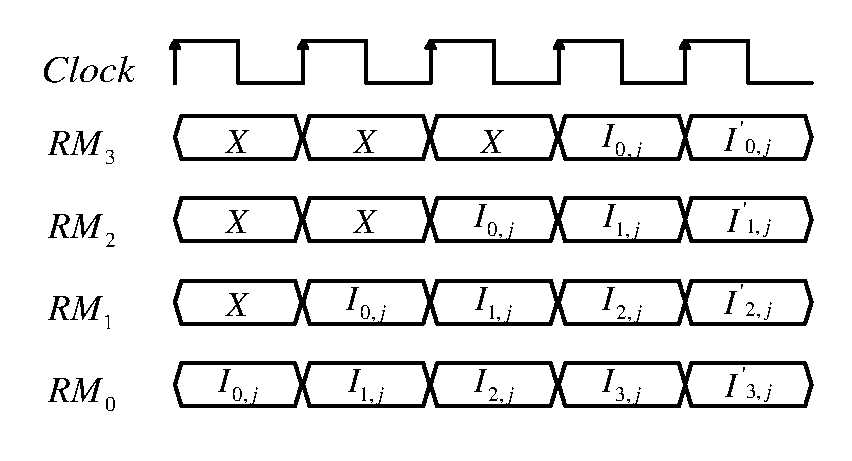
\includegraphics[width=0.45\textwidth]{./fig/Mix-Columns-Times.pdf}
    \caption{Timing Diagram for the Serial Architecture of Mix-Columns }\label{serial_time_diagrm_mix_colunms}
\end{figure}

\subsubsection{Control Units}\label{subsubsec3}

The finite-state machine (FSM) of the serial architecture, as shown in Figure~\ref{serial_fsm_fig}, begins its encryption process by storing the initial key and plaintext in the Key-Register and State-Register, respectively.
The key undergoes expansion in the Key-Schedule phase, during which the clocks of the Mix-Columns and State-Register are disabled.
The Mix-Columns phase follows, storing one column of the State-Register in the Mix-Columns registers and taking five clock cycles to execute Mix-Columns on one column.
Upon completion of this phase, the clocks of the State-Register and Key-Register are disabled.
The Sub-Box phase then takes over, sending the data stored in the Mix-Columns registers back to the State-Register and XORing it with the keys, a process that takes another four clock cycles.
This cycle between the Mix-Columns and Sub-Box phases is repeated four times for the four columns of the State-Register.
The Permute operation is then executed in one clock cycle inside the State-Register.
The encryption process concludes when the Round counter reaches 31, at which point the ciphertext is stored in the State-Register.

\begin{figure}[h]%   
    \centering
    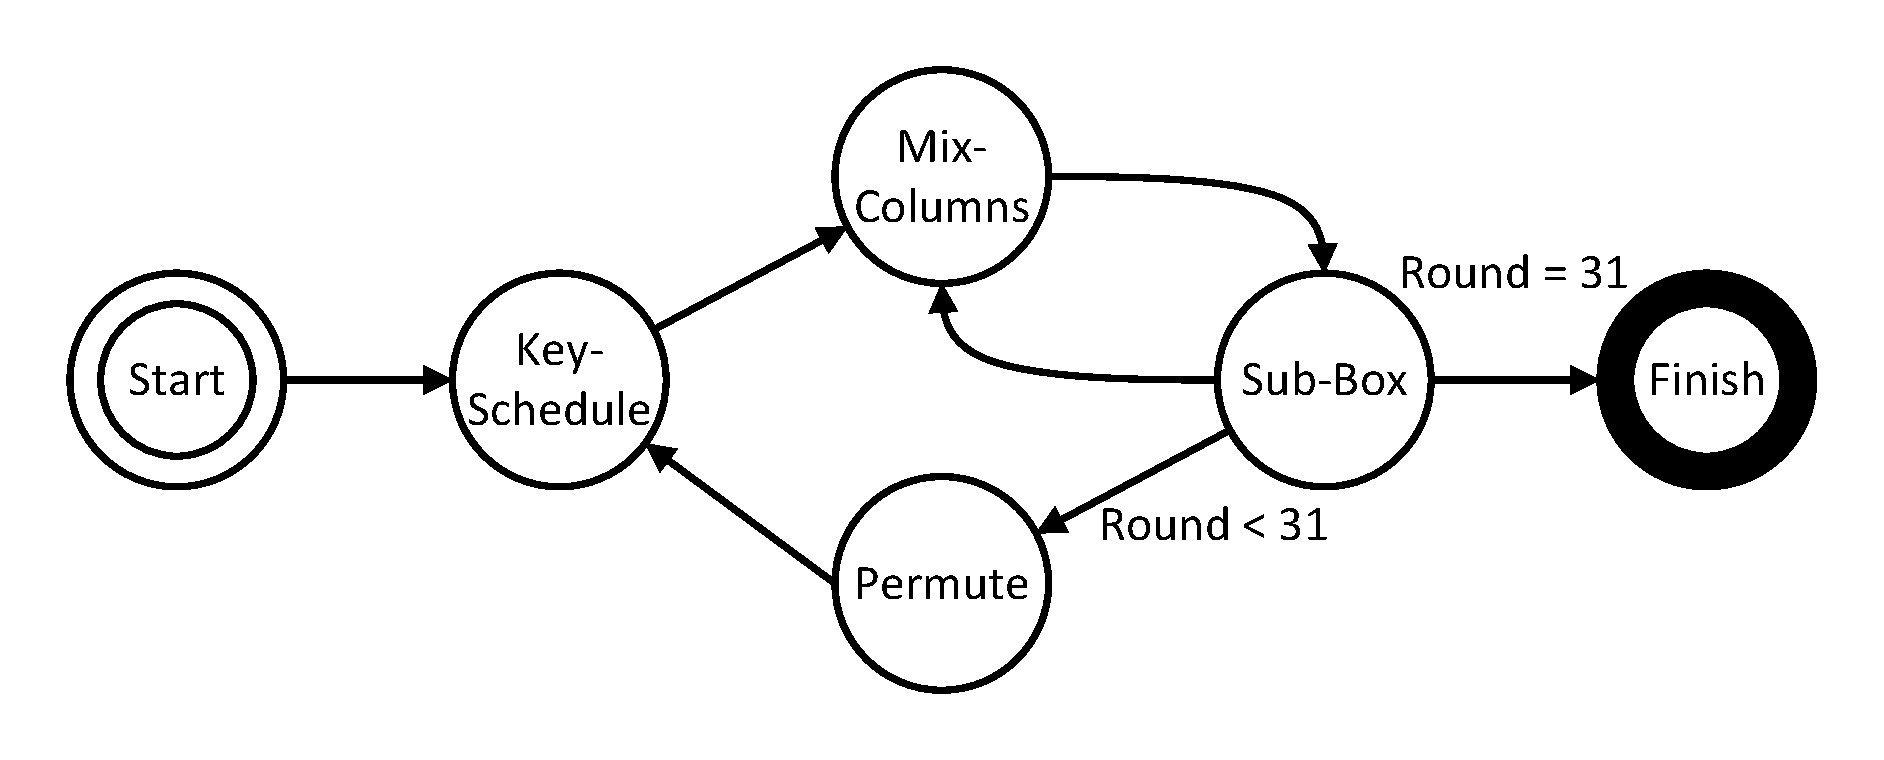
\includegraphics[width=0.45\textwidth]{./fig/serial-fsm.pdf}
    \caption{Finite-state machine for Serial Architecture}\label{serial_fsm_fig}
\end{figure}

Clock gating, a technique discussed in \cite{shahbazi2020area}, can help reduce the dynamic power consumption of the encryption.
This technique is applied separately to the State-Register, Key-Register, and Mix-Columns.
For example, during the Key-Schedule phase, the clock of the State-Register and Mix-Columns is turned off because these two blocks are not needed.
This helps save a significant amount of power. Figure~\ref{serial_time_diagrm} shows the timing diagram of a design that uses the clock gating technique.

\begin{figure}[h]%   
    \centering
    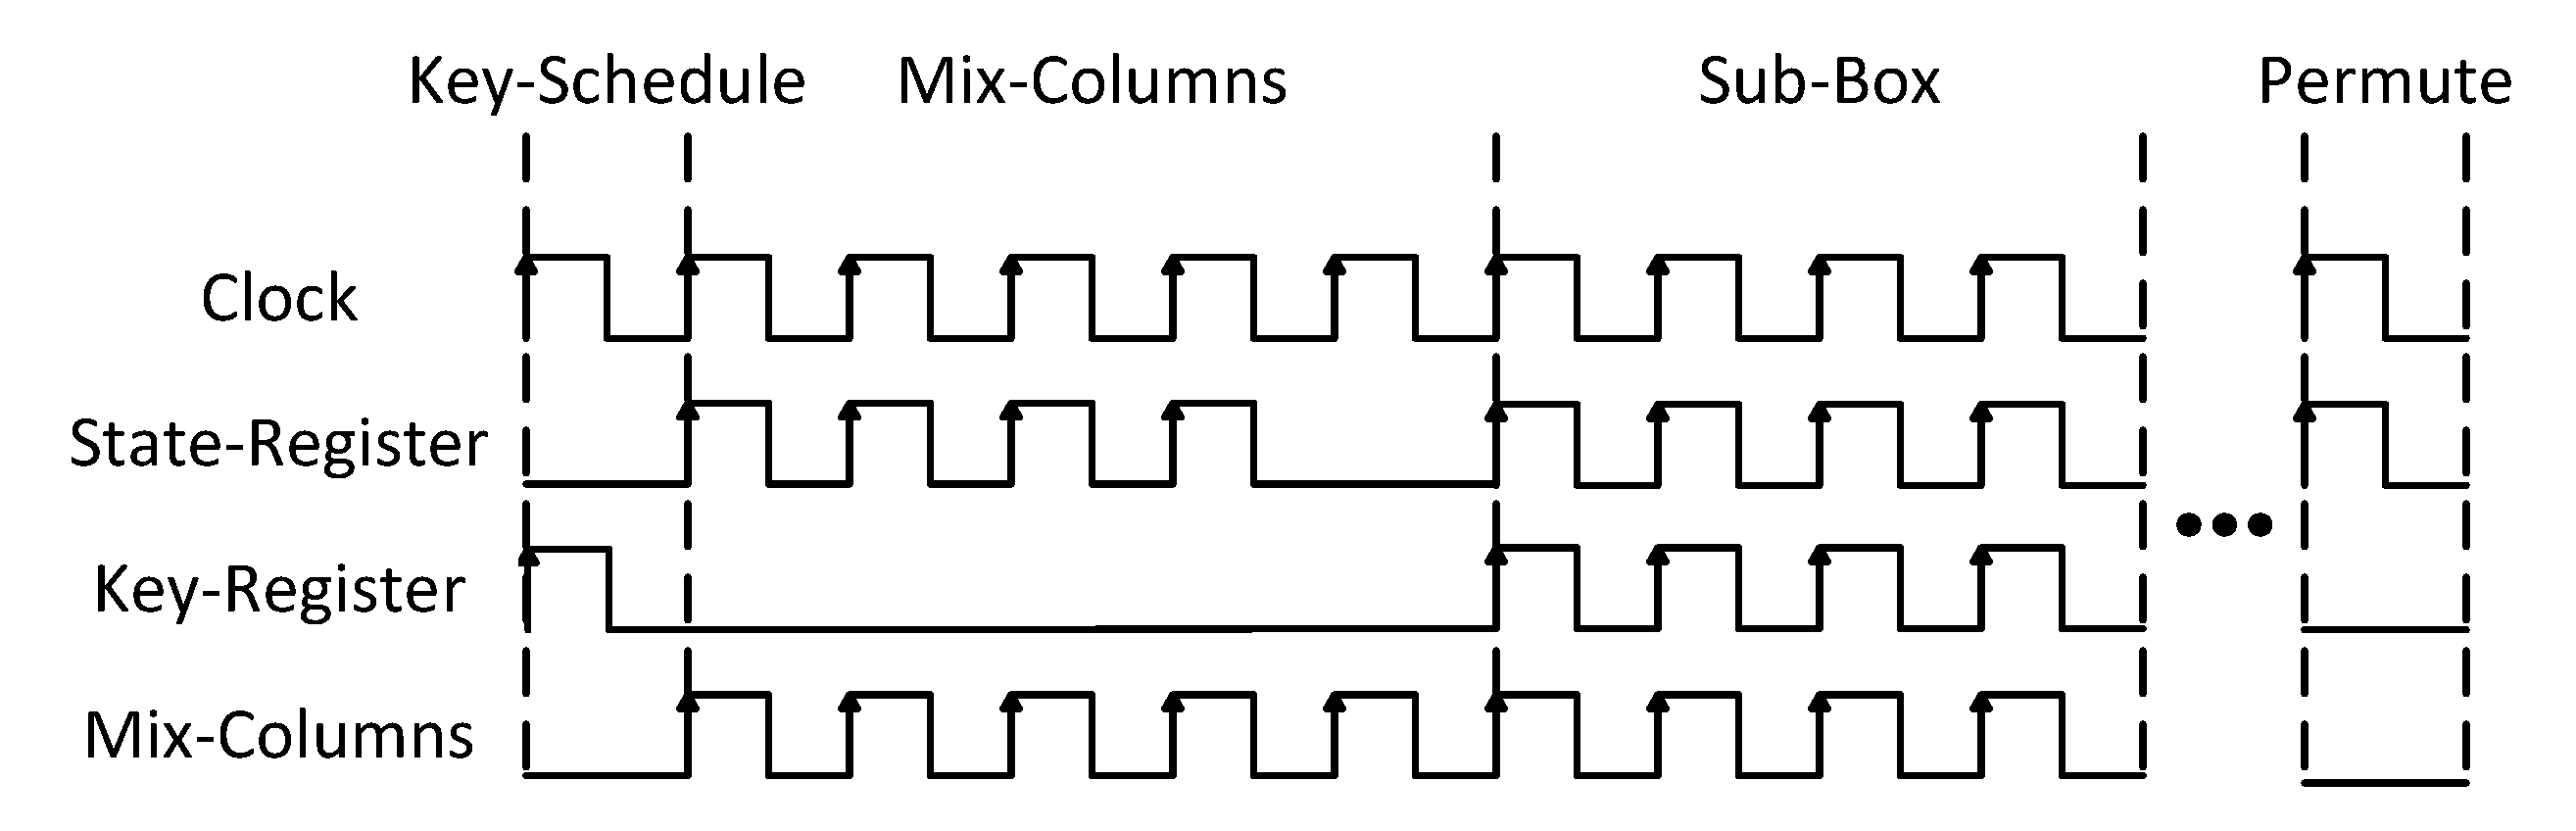
\includegraphics[width=0.45\textwidth]{./fig/serial-time.pdf}
    \caption{Timing diagram for Serial Architecture}\label{serial_time_diagrm}
\end{figure}
\subsection{Unrolled Architecture (A2)}\label{subsec3}

The architecture shown in Figure~\ref{fig4} includes two Sub-Boxes, two Mix-Columns, a Key, a State-Register, two PermuteNibbles, and one feedback path. It's designed to perform a 30-round encryption process in just 15 cycles. Only the Mix-Columns and Add-Key operations are carried out in the final cycle, finishing the encryption process in a total of 16 cycles.

The unrolled architecture, based on the iterative architecture from \cite{Beierle2019}, completes the encryption process in only 16 cycles, compared to the 32 cycles needed by the iterative architecture. Here, a cycle includes two round functions of CRAFT. While this approach might use more area, it provides higher throughput at the same frequency.


\begin{figure*}[h]%   
    \centering
    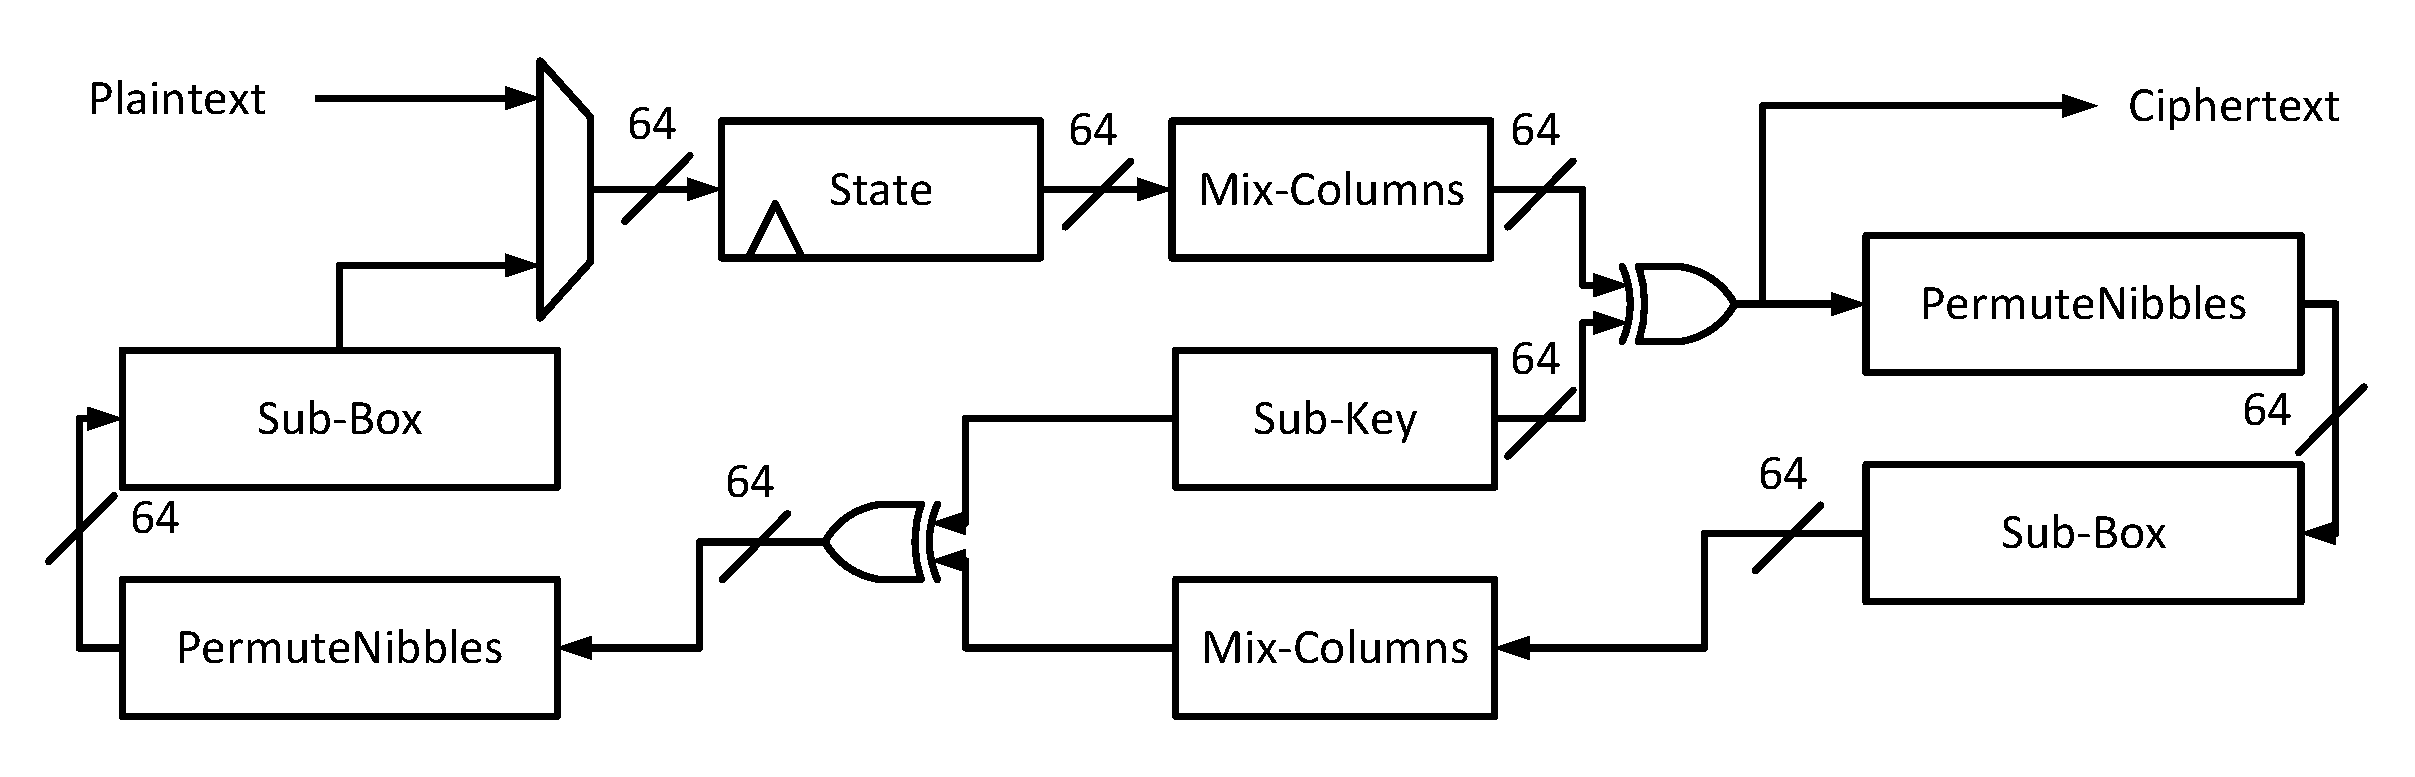
\includegraphics[width=0.7\textwidth]{./fig/unrolled-archticture.pdf}
    \caption{Unrolled architecture of CRAFT}\label{fig4}
\end{figure*}

\subsection{Iterative Architecture (A3)}\label{iterative_architecture}

The architecture from \cite{Bharathi2022} operates on a round-based architecture.
It employs a single round function to encrypt a block, incorporating a Sub-Box, a Permute, and an Add-Key operation.
This round function is executed 32 times to encrypt a single block. Concurrently, the Key Schedule runs alongside the round function.
This architecture is depicted in Figure~\ref{fig5}.
For comparison, different architectures are listed in Table~\ref{tab2}.

\begin{figure*}
    \centering
    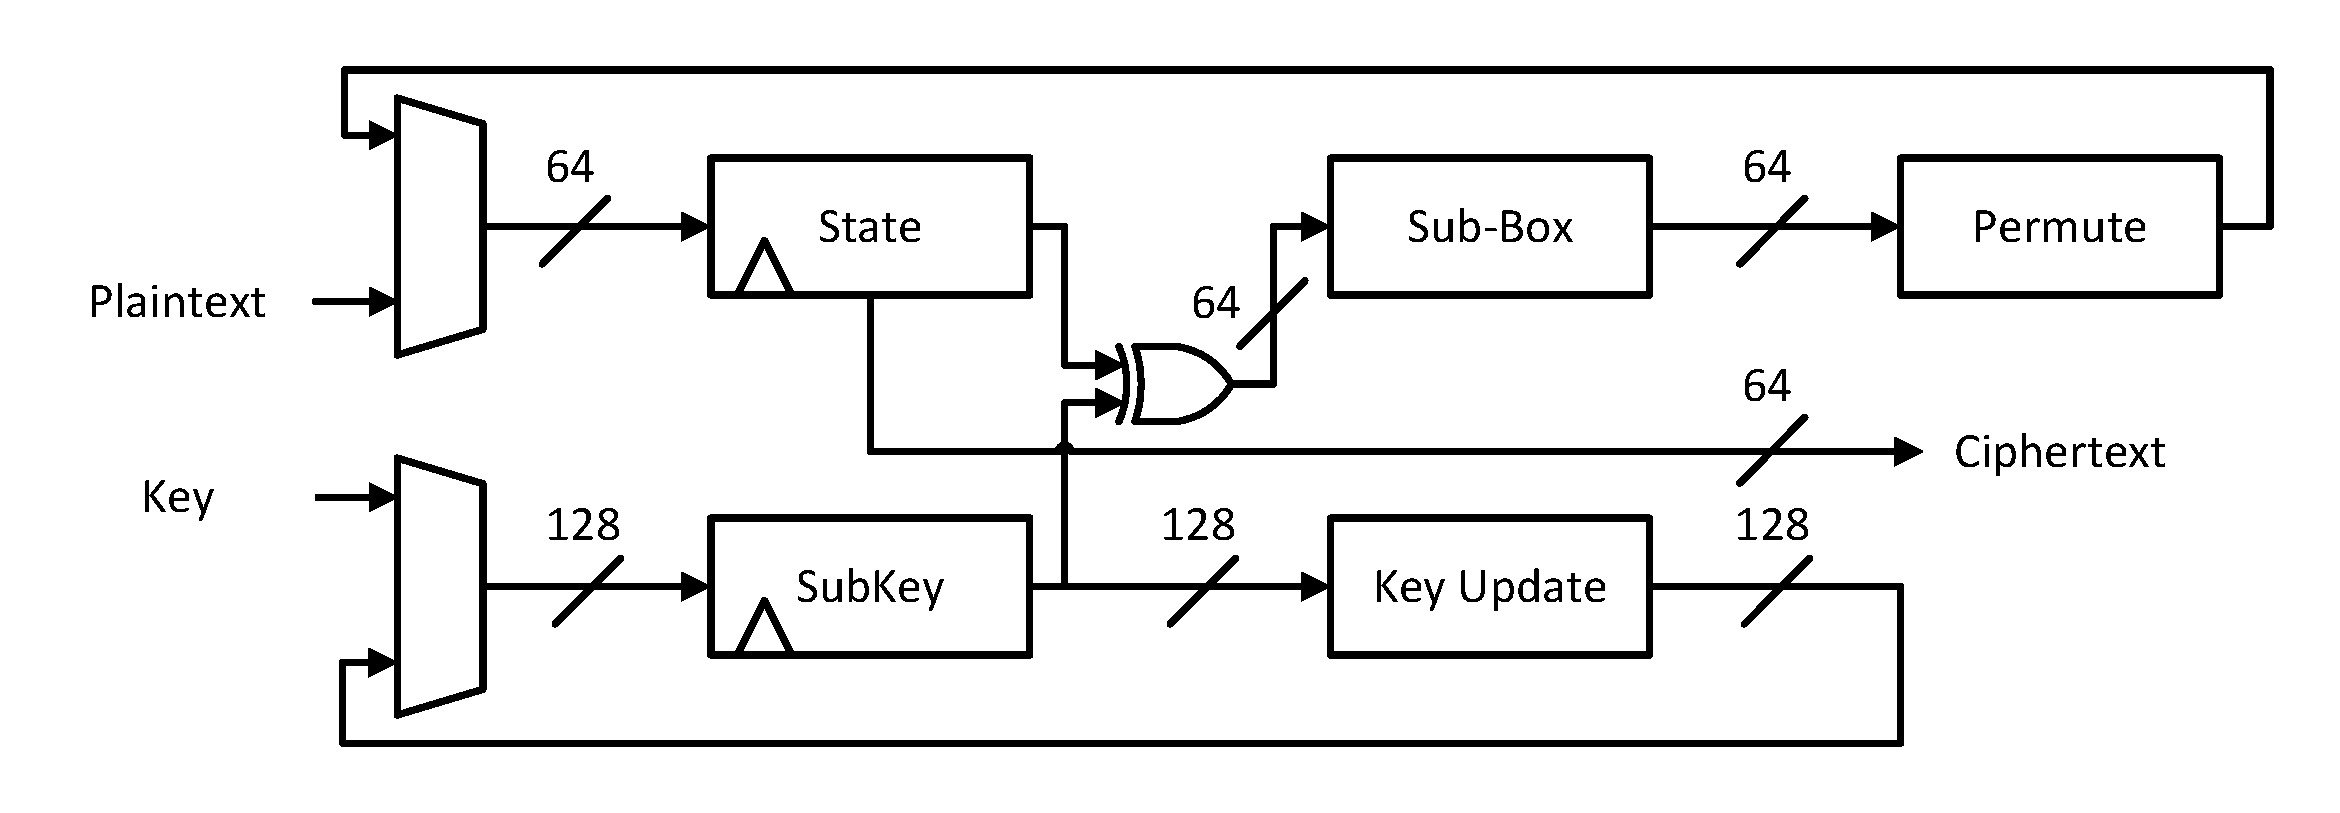
\includegraphics[width=0.75\textwidth]{./fig/iteration-present.pdf}
    \caption{Iterative architecture of PRESENT}\label{fig5}
\end{figure*}

\begin{table}[h]
    \centering
    \caption{Different architectures description}\label{tab2}%
    \begin{tabular}{|c|c|c|c|}
        \hline
        Architecture & Cipher  & Description & Reference           \\
        \hline
        A1           & CRAFT   & Serial      & This work           \\
        A2           & CRAFT   & Unrolled    & This work           \\
        A3           & PRESENT & Iterative   & \cite{Bharathi2022} \\
        \hline
    \end{tabular}
\end{table}


\section{Experimental Evaluation}\label{sec4}

In ASIC implementations, the gate equivalent (GE) is often used to evaluate the area consumption of a design.
A single GE is equivalent to a two-input NAND gate.
To calculate the area in GE, we divide the total area (in $\mu m^2$) by the area of a two-input NAND gate (also in $\mu m^2$).
However, the number of GEs can vary based on the specific technology used, as discussed in \cite{Turan}.
For instance, the number of GEs for the same design will differ between UMC 180nm technology and TSMC 180nm technology.
Therefore, GE is not suitable for comparing the area consumption of different designs on different technologies.
In order to ensure a fair comparison, we evaluate the area consumption of the proposed designs using FPGA implementations, a method also utilized in \cite{Mohajerani2020}.

\subsection{Platform}\label{subsec4}

The proposed architectures were implemented on a Xilinx FPGA board using Vivado v2023.2. To test in various environments, three different FPGA platforms were used for benchmarking: Artix-7(xc7a100tcsg324-1), Kintex-7(xc7k70tfbg484-1), and Spartan-7(xc7s100fgga484-1).
Artix-7 offers high performance in resource-limited situations. Spartan-7 is designed for high-restriction environments. Kintex-7 is ideal for applications like 3G and 4G wireless, flat panel displays, and video over IP solutions.


\subsection{Area}\label{subsec5}

The Area metric, which includes components like Flip-Flops, LUTs, and Slices, is used to measure the area used by the proposed designs. To make a fair comparison, the FPGA's embedded memory blocks were not used. This was done by turning off the related settings in the VHDL, as suggested in \cite{xilinx2022ultrafast}. Also, all designs were synthesized and implemented using the same settings, specifically, the default settings of Vivado Synthesis and Implementation.

\subsection{Throughput}\label{subsec6}
The performance of the proposed designs is evaluated using the Throughput metric. This metric uses three parameters: the maximum throughput rate, the throughput rate at 100MHz, and the throughput rate per slice.
The maximum throughput rate is the highest rate that our designs can achieve, calculated using Equation~\ref{eq4}.
The throughput rate at 100MHz shows the rate achievable when the clock frequency is set to 100MHz, calculated using Equation~\ref{eq5}.
The throughput rate per slice is a measure of efficiency, calculated by dividing the throughput rate by the number of Slices (Equation~\ref{eq6}).
In these calculations, the Plaintext Size is 64-bit, Latency refers to the number of clock cycles required to encrypt a single block, and Slices refers to the number of Slices used by the design.

\begin{equation}
    MaxThroughput(Thr) = \frac{MaxFrequency \times Plaintext Size}{Latency}
    \label{eq4}
\end{equation}

\begin{equation}
    Throughput_{@100MHz}(Thr^*) = \frac{100MHz \times Plaintext Size}{Latency}
    \label{eq5}
\end{equation}

\begin{equation}
    ThroughputPerSlice = \frac{Thr}{Slices}
    \label{eq6}
\end{equation}

\subsection{Power and Energy}\label{power_energy}

The Power metric, which includes both dynamic and static power consumption, is used to evaluate the power consumption of the proposed designs, as defined in Equation~\ref{eq7}.
On the other hand, the Energy metric measures the energy consumption of the designs. It's calculated by multiplying the power consumption by the time needed to encrypt a single block. This time is determined by dividing the latency by the frequency, as explained in Equation~\ref{enery_eqation}.

\begin{align}
    \text{Total Power} (TP) & = \text{Dynamic Power} (DP) \nonumber \\
                            & + \text{Static Power} (SP)
    \label{eq7}
\end{align}
\begin{equation}
    Energy(E) = \frac{TP \times Latency }{Frequency}
    \label{enery_eqation}
\end{equation}


\section{Results}\label{sec5}

This section presents the results of the proposed designs, divided into three categories: area, throughput, and power and energy. The results are demonstrated across three different FPGA platforms: Artix-7, Kintex-7, and Spartan-7. The area consumption of the designs is displayed in Table~\ref{area_compare}, the throughput results are illustrated in Table~\ref{throughput_compare}, and the details of power and energy consumption are provided in Table~\ref{power_energy_compare}.


\begin{table*}[h]
    \caption{Area used for the three Architectures}\label{area_compare}%
    \begin{tabular*}{\textwidth}{@{\extracolsep\fill}|c|c|c|c|c|c|c|}
        \hline
        Platform & Design & $State(bit)$ & $Key(bit)$ & $FF$ & $LUT$ & $Slices$ \\
        \hline
        \multirow{3}{*}{Artix-7}  & A1 & 64 & 128 & \textbf{144} & \textbf{177} & \textbf{59} \\
        & A2 & 64 & 128 & 157 & 378 & 111 \\
        & A3 & 64 & 128 & 201 & 243 & 70 \\
        \hline
        \multirow{3}{*}{Kintex-7} & A1 & 64 & 128 & \textbf{144} & \textbf{178} & \textbf{58}\\
        & A2 & 64 & 128 & 157 & 377 & 115 \\
        & A3 & 64 & 128 & 201 & 244 & 68 \\
        \hline
        \multirow{3}{*}{Spartan-7} & A1 & 64 & 128 & \textbf{144} & \textbf{177} & \textbf{57}\\
        & A2 & 64 & 128 & 157 & 381 & 118 \\
        & A3 & 64 & 128 & 201 & 244 & 70 \\
        \hline
    \end{tabular*}
\end{table*}

\begin{table*}
    \begin{threeparttable}
        \caption{Throughput results for the three Architectures}\label{throughput_compare}%
        \begin{tabular*}{\textwidth}{@{\extracolsep\fill}|c|c|c|c|c|c|c|}
            \hline
            Platform & Design & $Latency$ & $MaxF(MHz)$ & $Thr(Mbps)$ & $Thr^*(Mbps)$\tnote{a} & $Thr/Slices$($Kbps/Slices$) \\
            \hline
            \multirow{3}{*}{Artix-7}  & A1 & 1215 & \textbf{557.41} & 29.36 & 5.27 & 497.65 \\
            & A2 & \textbf{16} & 142.38 & 569.52 & \textbf{400.00} & 5130.81 \\
            & A3 & 32 & 274.04 & 548.08 & 200.00 & 7829.71 \\
            \hline
            \multirow{3}{*}{Kintex-7} & A1 & 1215 & \textbf{853.97} & 44.98 & 5.27 & 775.57 \\
            & A2 & \textbf{16} & 175.25 & 701.00 & \textbf{400.00} & 6095.65 \\
            & A3 & 32 & 357.78 & 715.56 & 200.00 & 10522.94 \\
            \hline
            \multirow{3}{*}{Spartan-7} & A1 & 1215 & \textbf{525.76} & 27.69 & 5.27 & 485.87 \\
            & A2 & \textbf{16} & 138.86 & 555.44 & \textbf{400.00} & 4707.12 \\
            & A3 & 32 & 296.29 & 592.58 & 200.00 & 8465.43 \\
            \hline
        \end{tabular*}
        \begin{tablenotes}
            \item[a] Throughput rate at 100MHz
        \end{tablenotes}
    \end{threeparttable}
\end{table*}

\begin{table*}
    \begin{threeparttable}
        \caption{Power and Energy consumption for the three Architectures}\label{power_energy_compare}%
        \begin{tabular*}{\textwidth}{@{\extracolsep\fill}|c|c|c|c|c|c|c|}
            \hline
            Platform & Design & $DP(mW)$ & $SP(mW)$ & $TP(mW)$ & $E(uJ)$ & $E/bit(nJ/bit)$ \\
            \hline
            \multirow{3}{*}{Artix-7}  & A1 & 2.00 & 139.00 & 141.00 & 1.71 & 26.77 \\
            & A2 & 7.00 & 139.00 & 146.00 & \textbf{0.02} & \textbf{0.37} \\
            & A3 & 2.00 & 139.00 & 141.00 & 0.05 & 0.71 \\
            \hline
            \multirow{3}{*}{Kintex-7} & A1 & 2.00 & 145.00 & 147.00 & 1.79 & 27.91 \\
            & A2 & 8.00 & 145.00 & 153.00 & \textbf{0.02} & \textbf{0.38} \\
            & A3 & 3.00 & 145.00 & 148.00 & 0.05 & 0.74 \\
            \hline
            \multirow{3}{*}{Spartan-7} & A1 & 2.00 & 140.00 & 142.00 & 1.73 & 26.96 \\
            & A2 & 7.00 & 140.00 & 147.00 & \textbf{0.02} & \textbf{0.37} \\
            & A3 & 3.00 & 140.00 & 143.00 & 0.05 & 0.72 \\
            \hline
        \end{tabular*}
        \begin{tabular}{llll}
            DP: Dynamic Power & SP: Static Power & TP: Total Power & E: Energy
        \end{tabular}
    \end{threeparttable}
\end{table*}

The area consumption of the proposed designs is evaluated based on three factors: Flip-Flops (FF), Look-Up Tables (LUT), and Slices. These designs are compared with the iterative architecture of PRESENT (A3) , as described in \cite{Bharathi2022}. The results indicate that the proposed designs consume 15.72\% less area than the iterative architecture of PRESENT.

Regarding the Flip-Flops (FF), the key schedule of the CRAFT cipher is implemented using multiplexers. This eliminates the need for FF to store the sub-key, resulting in a lower FF count compared to other ciphers. This is a significant factor contributing to the CRAFT cipher's requirement of less than 1000 GE, which is the lowest known requirement on the IBM 130 nm ASIC library, as shown in \cite{Beierle2019}. A comparison of FF counts is provided in Figure~\ref{compare_ff}.

\begin{figure}
    \centering
    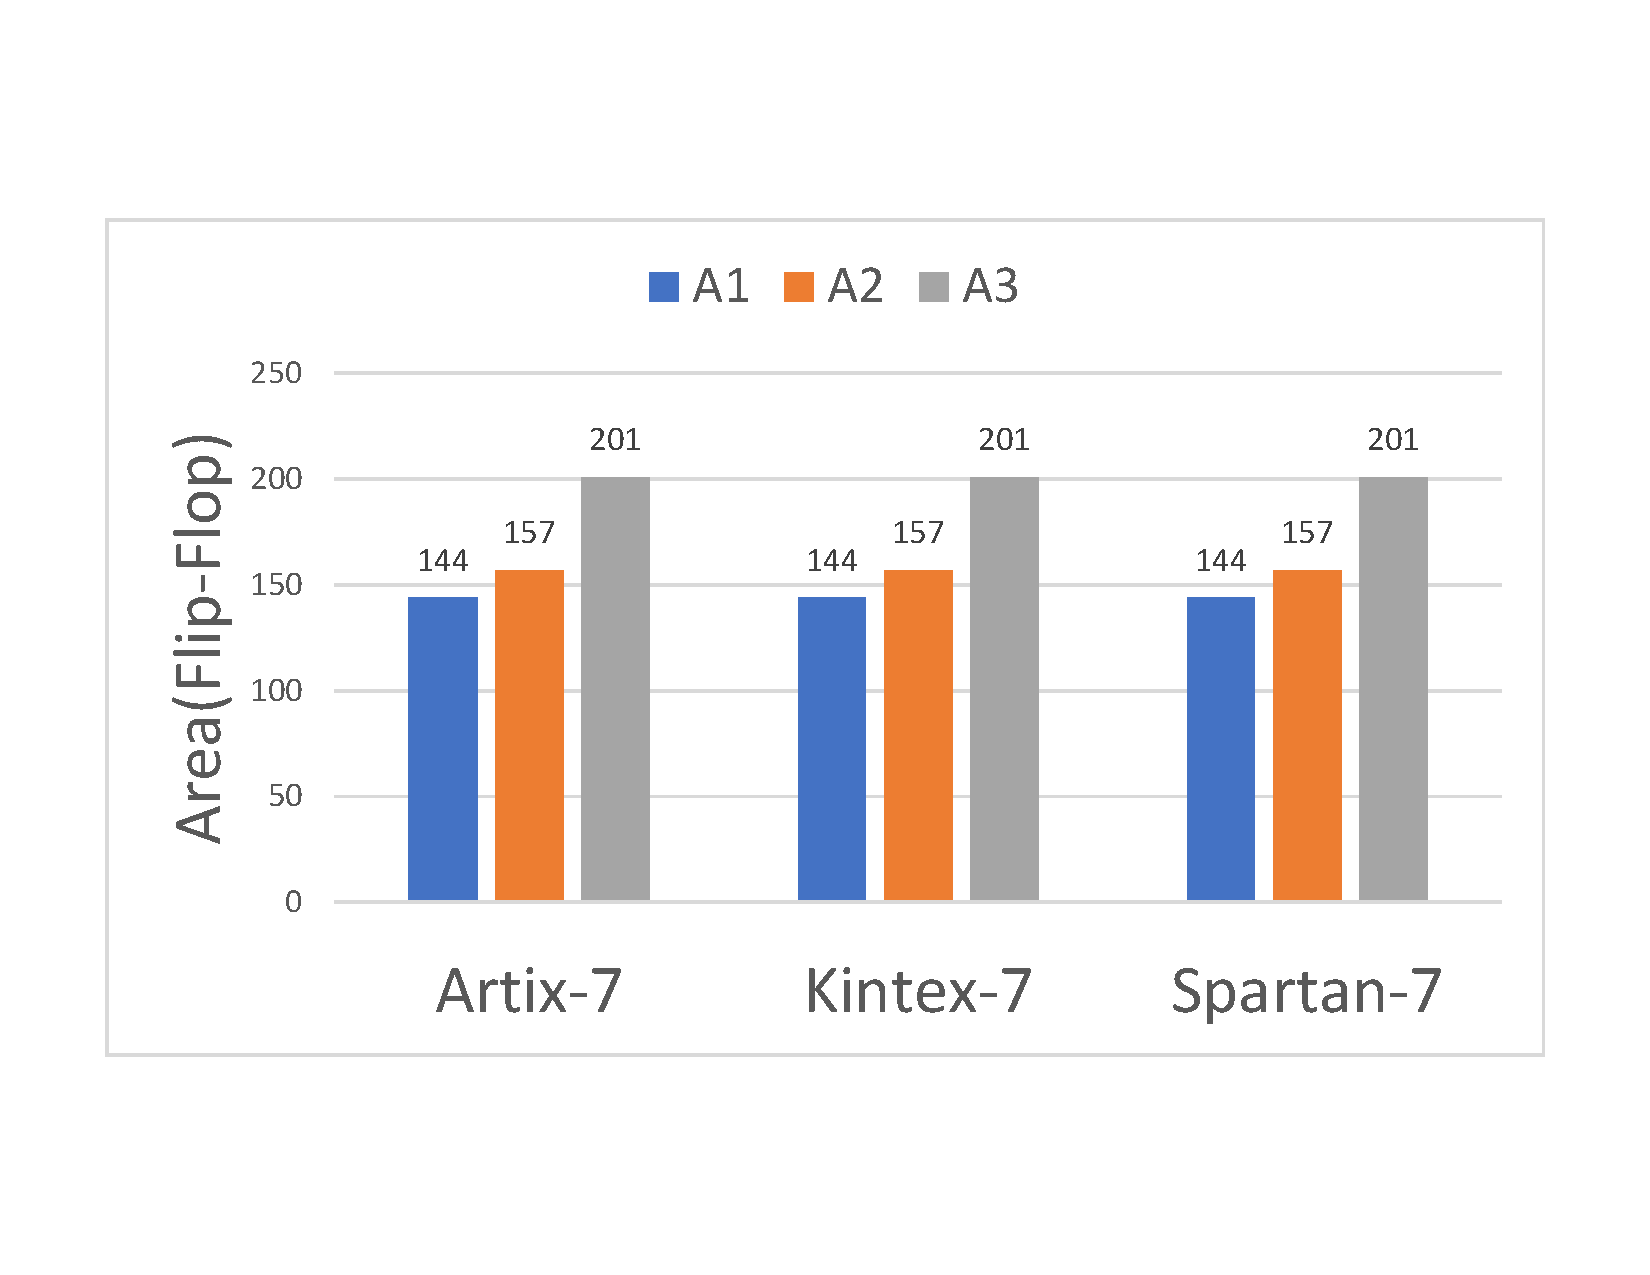
\includegraphics[width=0.45\textwidth]{./fig/compare-ff.pdf}
    \caption{Comparison of Flip-Flop in three Architectures}\label{compare_ff}
\end{figure}

As illustrated in Figure~\ref{compare_lut}, when it comes to Look-Up Tables (LUT), the proposed designs (A1) require fewer LUTs than the iterative architecture of PRESENT (A3). This is attributed to the fact that the proposed designs utilize a single Sub-Box, in contrast to the 16 Sub-Boxes used by the iterative architecture of PRESENT. Furthermore, the proposed designs also require fewer LUTs than the unrolled architecture of CRAFT, which uses 32 Sub-Boxes, compared to just one in the proposed designs.

\begin{figure}
    \centering
    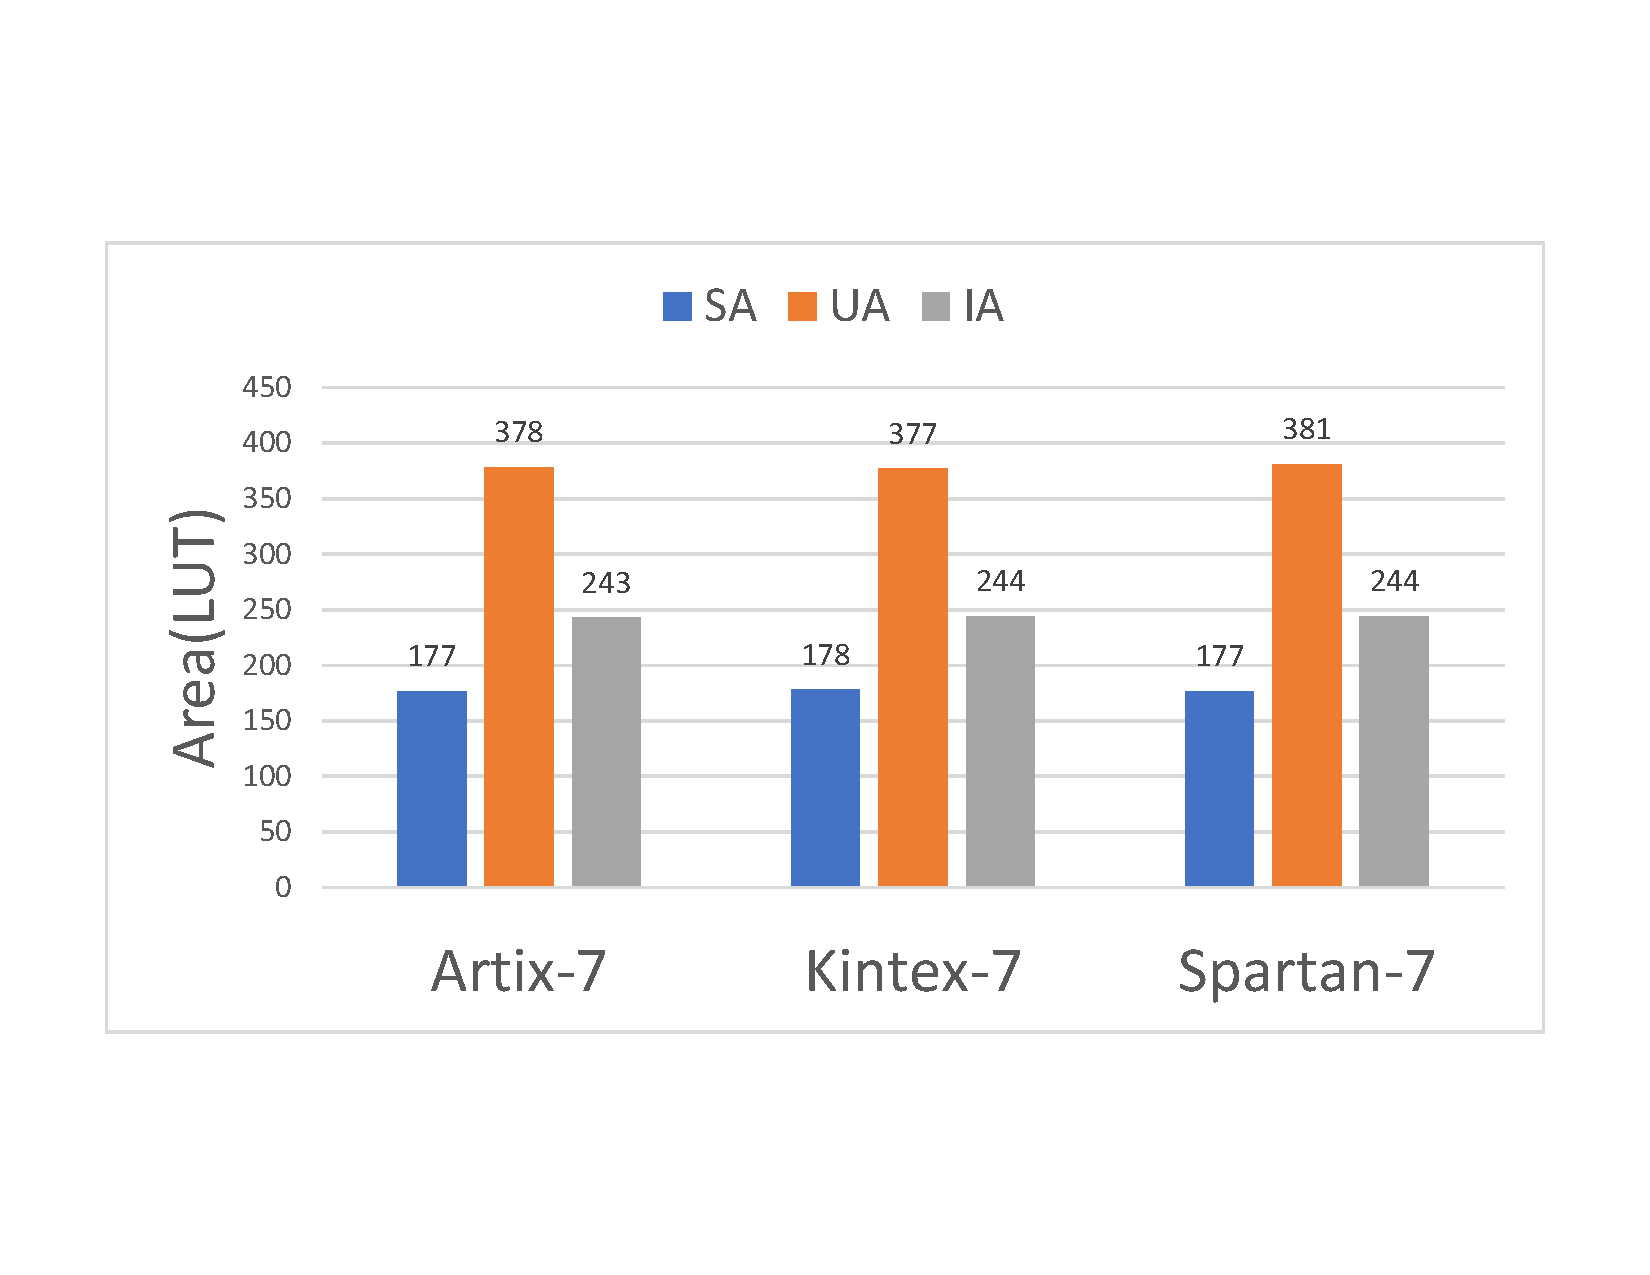
\includegraphics[width=0.45\textwidth]{./fig/compare-lut.pdf}
    \caption{Comparison of Look-Up Tables in three Architectures}\label{compare_lut}
\end{figure}

The serial architecture (A1) has a lower Slices cost compared to the iterative architecture of PRESENT (A3), thanks to the reduction in FF and LUT usage. Among the platforms, Spartan-7 is the most efficient in terms of Slices, followed by Artix-7 and Kintex-7. These results are illustrated in Figure~\ref{compare-slices}. However, the lower Max Frequency of Spartan-7 will be considered in the Throughput comparison.

\begin{figure}
    \centering
    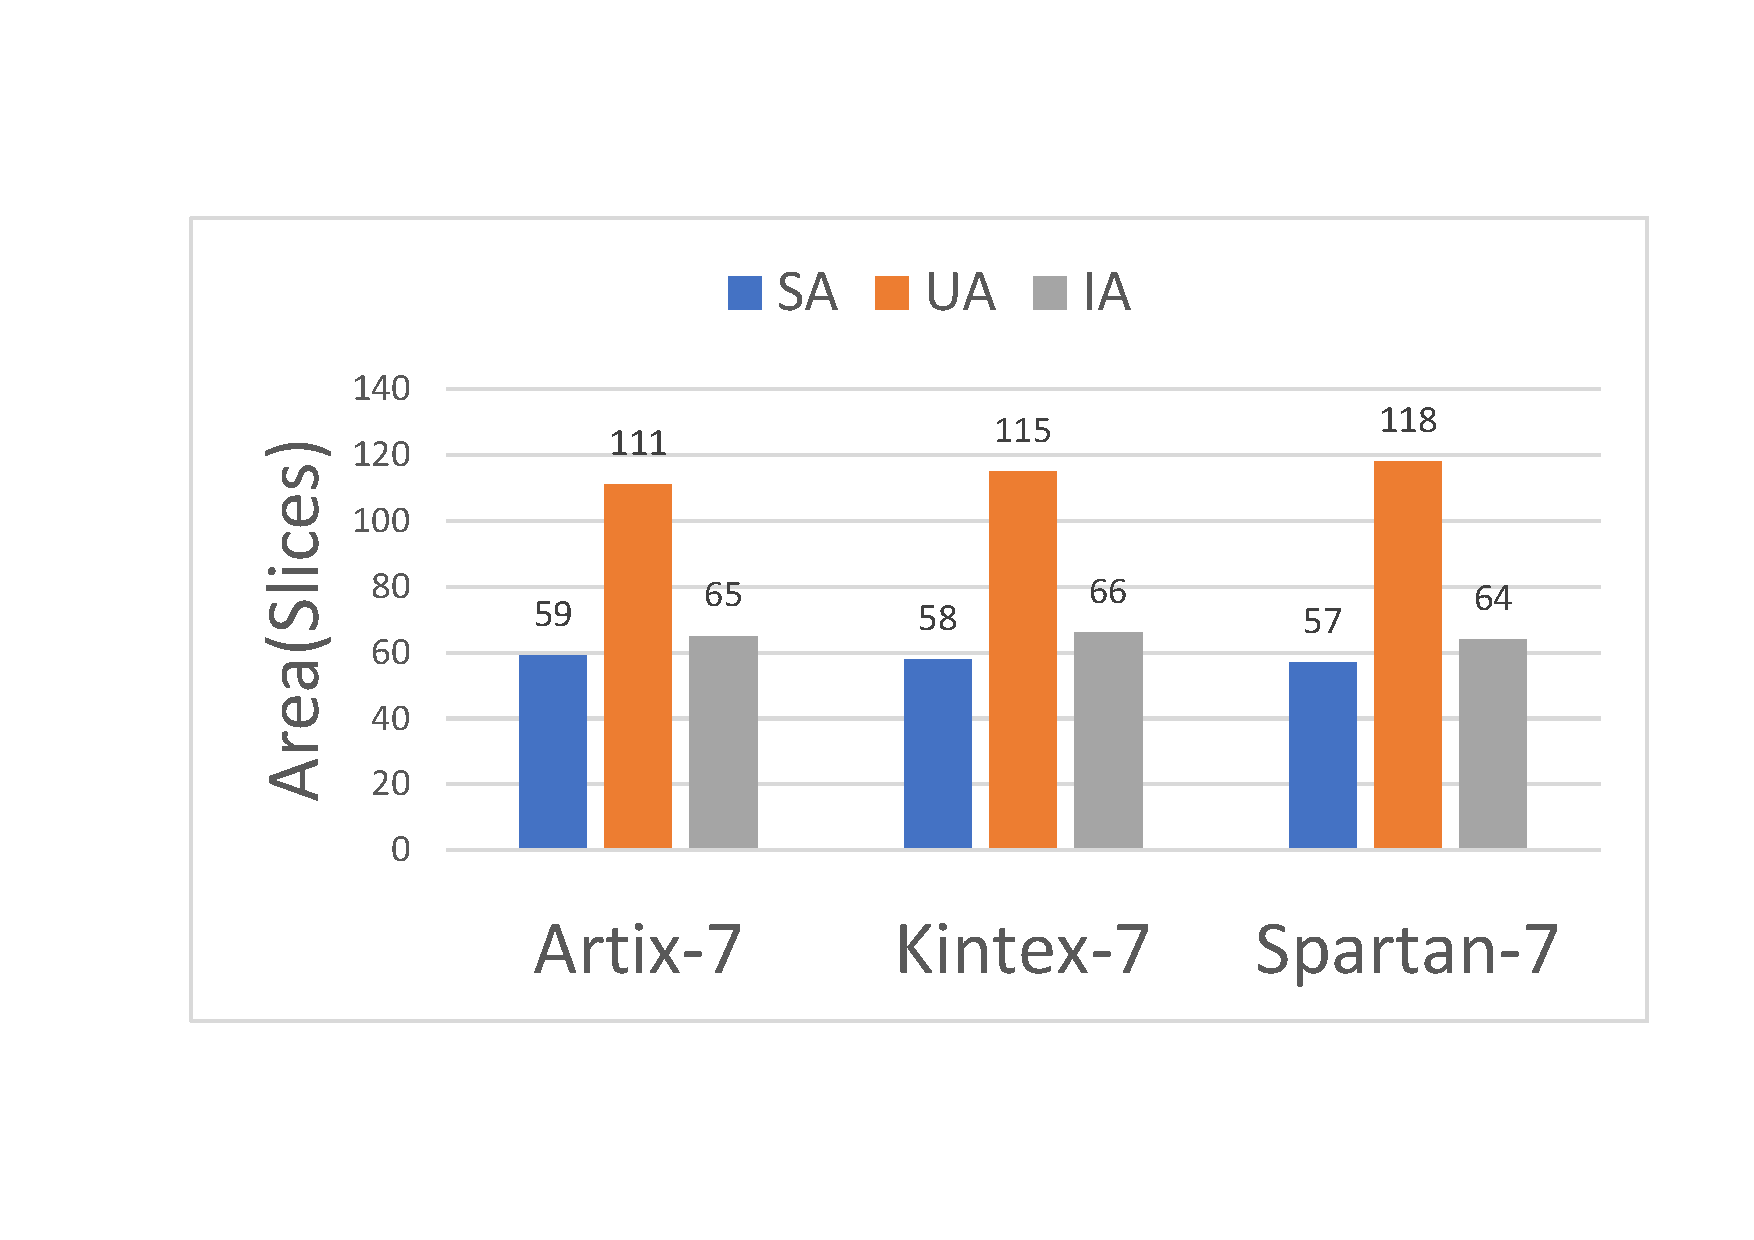
\includegraphics[width=0.45\textwidth]{./fig/compare-slices.pdf}
    \caption{Comparison of Slices in three Architectures}\label{compare-slices}
\end{figure}

Figure~\ref{compare-maxF} illustrates that the proposed designs (A1) have a higher Max Frequency than the iterative architecture of PRESENT (A3). This improvement is due to two key factors. First, the Sub-Box is optimized with the GEC encoding scheme, reducing its delay. Second, the serial architecture of the design further reduces the overall delay of the encryption process. However, among all platforms, Spartan-7 has the lowest Max Frequency, primarily because it has the fewest LUTs, as shown in Figure~\ref{compare_lut}. The unrolled architecture (A2) reduces the latency to 16, which doubles the Throughput rate at 100MHz compared to the iterative architecture of PRESENT (A3). This data is presented in Table~\ref{throughput_compare}.

\begin{figure}
    \centering
    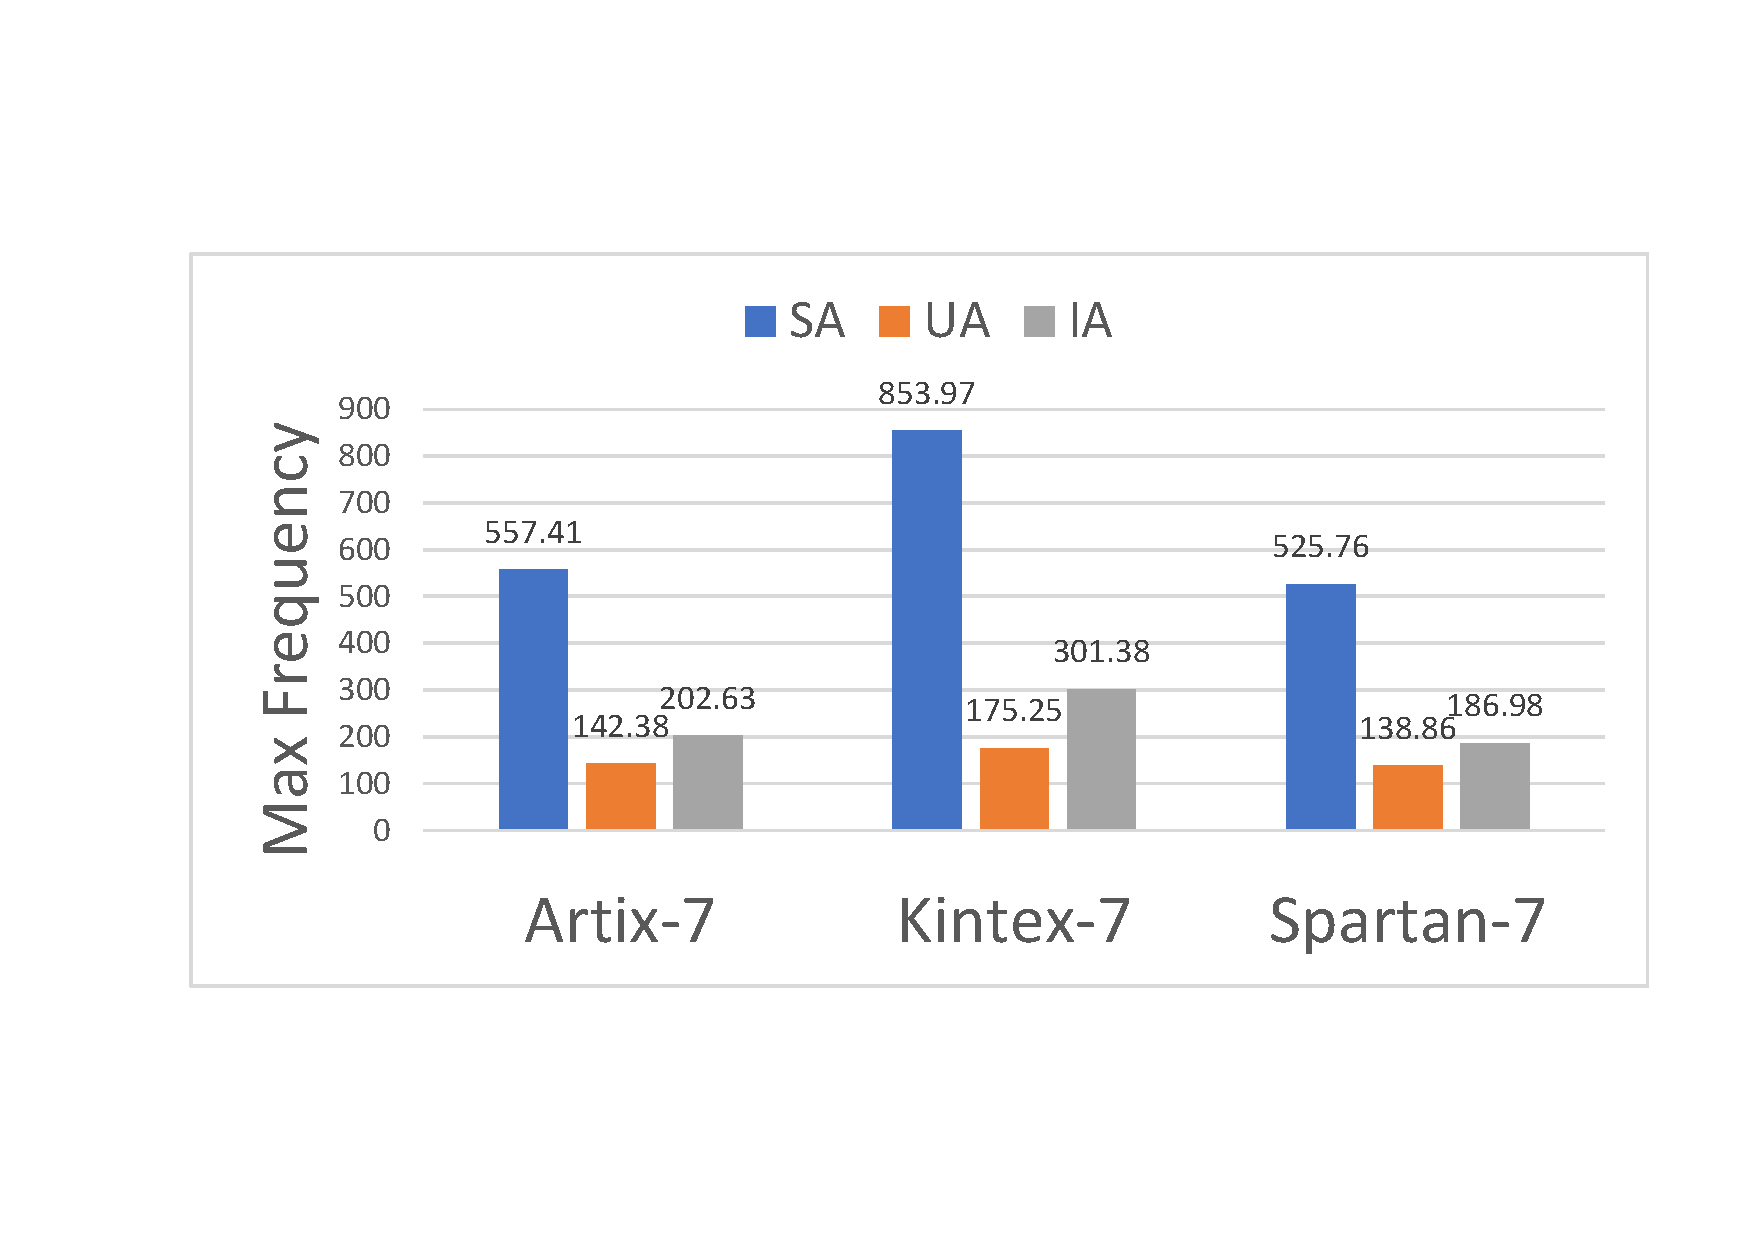
\includegraphics[width=0.45\textwidth]{./fig/compare-maxf.pdf}
    \caption{Comparison of Max Frequency in three Architectures}\label{compare-maxF}
\end{figure}

The serial architecture (A1) has the highest energy per bit due to its higher latency, which results in the smallest area. Conversely, the unrolled architecture (A2) has the lowest energy per bit because it has the lowest latency. The energy per bit of the iterative architecture of PRESENT (A3) falls between that of the serial architecture (A1) and the unrolled architecture (A2). Compared to the iterative architecture of PRESENT (A3), the unrolled architecture (A2) reduces energy per bit by 47.89\%. Figure~\ref{compare-energy} illustrates the energy per bit for the three architectures.

\begin{figure}
    \centering
    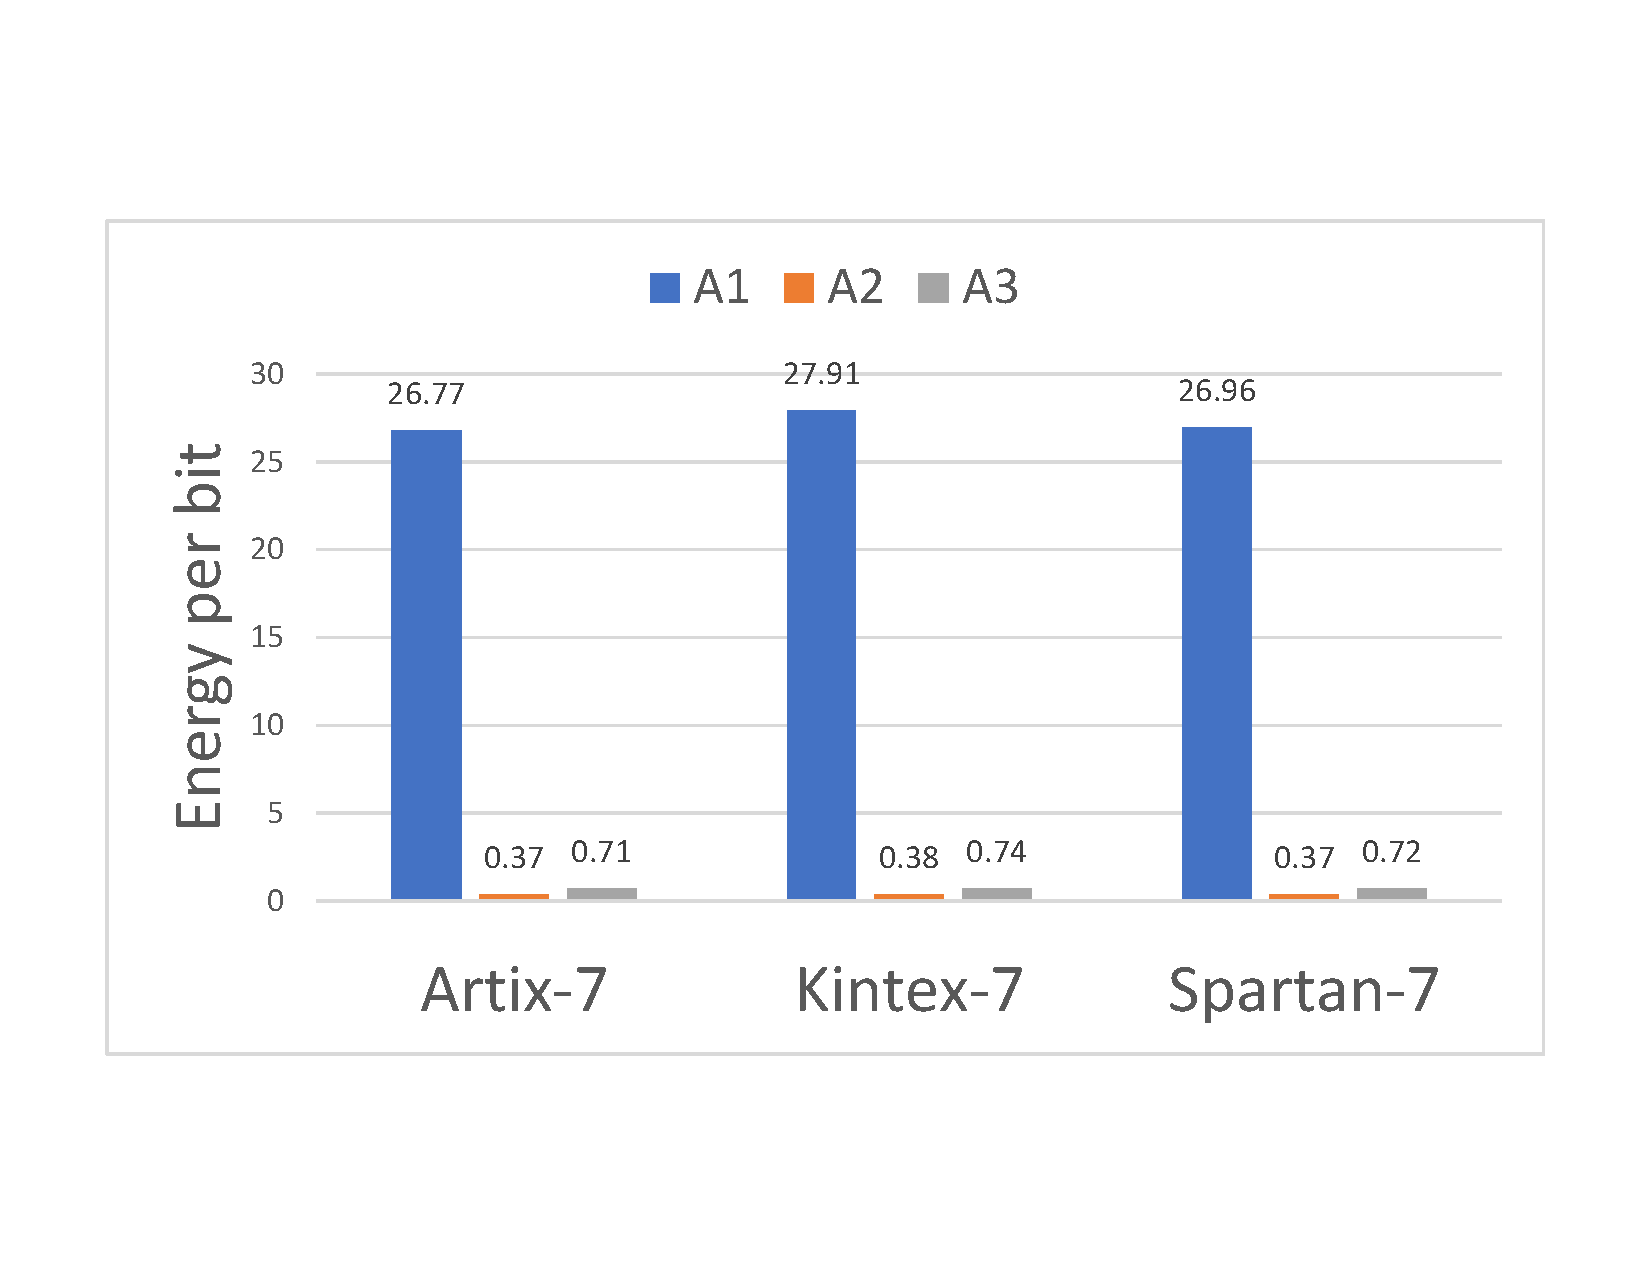
\includegraphics[width=0.45\textwidth]{./fig/compare-energy.pdf}
    \caption{Comparison of Energy per bit in three Architectures}\label{compare-energy}
\end{figure}


\section{Conclusion}\label{sec6}

The Internet of Things (IoT) has brought about a revolution in the interaction with devices and data, enabling unprecedented levels of connectivity and automation. However, the resource-constrained environments in which IoT devices often operate pose challenges for the implementation of robust security measures. Lightweight cryptographic algorithms, such as the CRAFT cipher, are crucial for ensuring these devices' security without overtaxing their limited resources.

This paper presents two architectures for the CRAFT cipher: Serial and Unrolled. The Serial architecture reduces the area consumption by 15.72\% compared to the iterative architecture of PRESENT. The Unrolled architecture, on the other hand, reduces the latency to 16, effectively doubling the throughput rate at 100MHz compared to the iterative architecture of PRESENT. Additionally, the Unrolled architecture reduces energy per bit by 47.89\% compared to the iterative architecture of PRESENT. These proposed architectures are well-suited for resource-constrained environments, such as those found in IoT devices.

Future work could involve investigating the application of these proposed architectures in real-world IoT devices and measuring their performance. Additionally, implementing these architectures on ASICs could further reduce area consumption.

\bibliographystyle{elsarticle-num}
\bibliography{bibliography}

\end{document}
\endinput
%%
%% End of file `elsarticle-template-num.tex'.
